\documentclass[12pt]{report}
\usepackage[margin=1in]{geometry}
\usepackage{hyperref}
\usepackage{graphicx}
\usepackage{amsmath}
\usepackage{enumitem}
\usepackage{float}

\title{Week 2 Report}
\author{Dhanush Balusa}
\date{May 27, 2025}

\begin{document}

\maketitle

\chapter*{Research}

Here are some notes/resources to patch up the concept gaps I had from week 1.\\

\textbf{TLE:}
\begin{itemize}
  \item \url{https://web.archive.org/web/20000301052035/http://spaceflight.nasa.gov/realdata/sightings/SSapplications/Post/JavaSSOP/SSOP_Help/tle_def.html}
  \item \url{https://www.mathworks.com/help/satcom/gs/satelliteScenario-key-concepts.html#mw_e08739b4-c5da-4983-898b-56e18cc71f87}
\end{itemize}

\textbf{Coordinate System: Geocentric Celestial Reference Frame}
\begin{itemize}
  \item X-axis: points toward the vernal equinox (the intersection of the Earth's equatorial plane and the ecliptic plane at J2000.0).
  \item Y-axis: lies in the equatorial plane and 90\textdegree{} east of the X-axis.
  \item Z-axis: points toward the Celestial North Pole (aligned with Earth's mean rotation axis at epoch J2000.0).
\end{itemize}

\textbf{SGP4:} units: metric\\

Other resources:
\begin{itemize}
  \item \url{https://celestrak.org/columns/v04n03/}
\end{itemize}

\chapter*{Previous Code}
My code from the previous week calculated the approach conditions between the ISS and NOAA 15.
\begin{figure}[H]
    \centering
    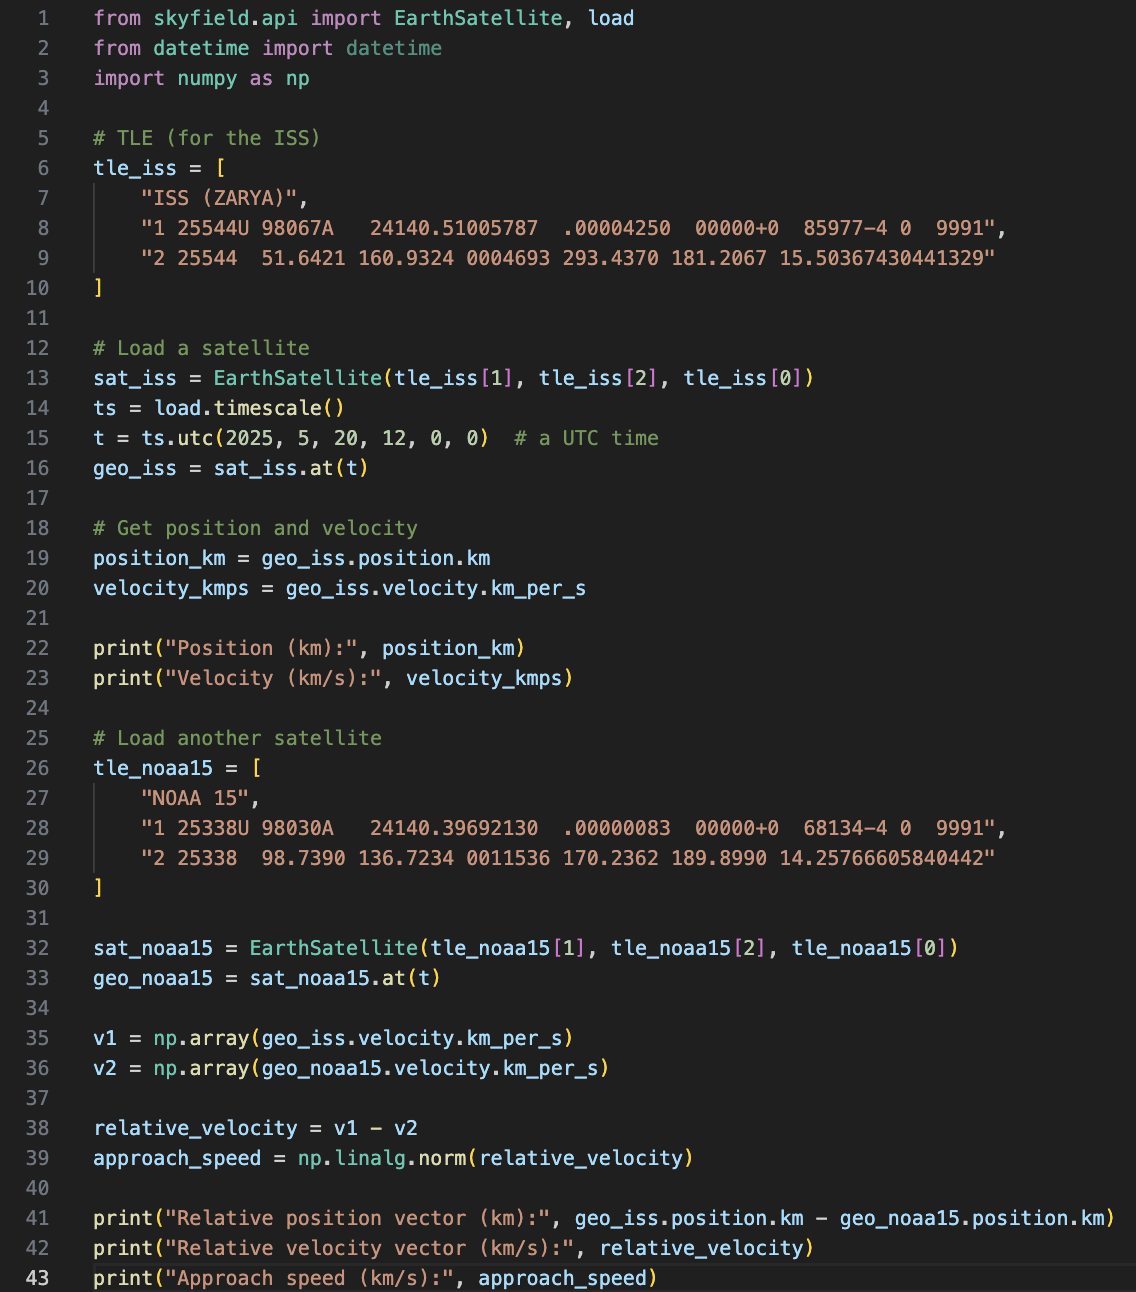
\includegraphics[width=0.8\textwidth]{figure_week_1_test_code.png}
    \caption{Test code from week 1 calculating the approach conditions between ISS and NOAA15}
    \label{fig:orbit}
\end{figure}

\chapter*{Code Changes}

Based on the feedback from last week’s team meeting, I decided to make the following changes:

\begin{enumerate}
  \item \textbf{My first change was to implement the space-track.org API to get TLE data}

  \textit{Issue:} The EarthSatellite (SGP4) wants 3 arguments but the API call only returns the 2 lines (not the satellite’s name).

  \textit{Fix:} However, I found out a work around be prepending the name:
  \begin{verbatim}
  tle_lines = fetch_tle(norad_id, username, password)
  tle_iss = ["ISS (ZARYA)"] + tle_lines
  \end{verbatim}
  Note: I need to check if the TLE data is fetched correctly.

  \item \textbf{My second change was to loop through a bunch of LEO satellites. I did this with an array of satellites and their catalog number.}

  Note: I need to loop through relevant satellites and potentially go through the whole database.

  \newpage
  \item \textbf{My third change was to loop through a wide time range.}

  \begin{figure}[H]
    \centering
    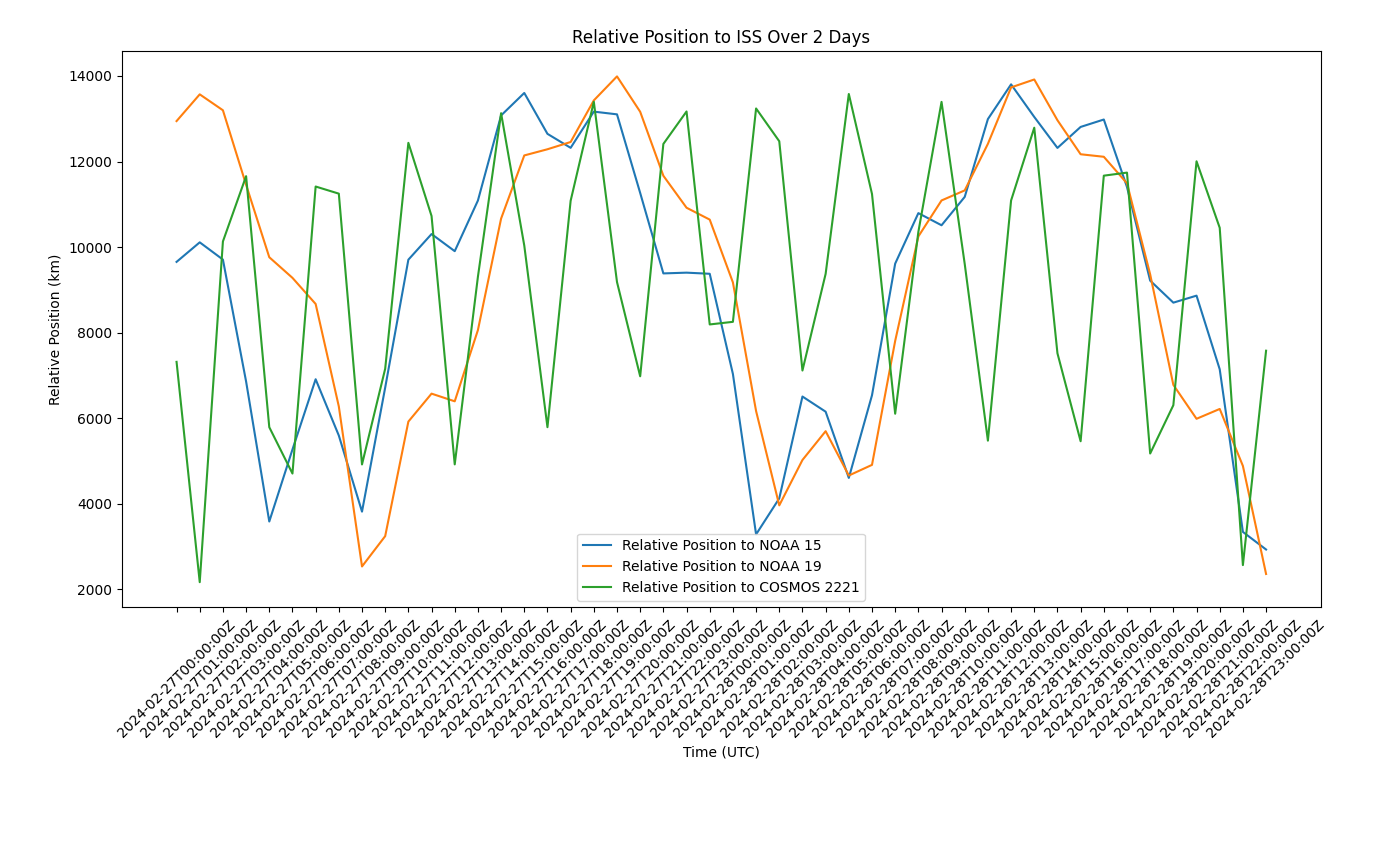
\includegraphics[width=0.8\textwidth]{figure_sats_looped.png}
    \caption{Relative position of ISS and other LEO satellites over time}
    \label{fig:orbit}
  \end{figure}


  \textit{Issue:} When I looped through a huge time range, the plot became very hard to read. However, this also seems to be because I am calculating the approach conditions wrong (more on this in \#5), so I need to go back and check if the SGP4 is working.

  \item \textbf{My fourth step is to graph the relative position vs time to find close approaches}

  \textit{Issue:} VS Code has a problem compiling the code but using Mac’s Terminal worked fine. I need to check which change I made in this step is causing VS Code to not compile.

  \textit{Improve:} Understand why the relative position is not periodic. Is it because of drag? Or the orbits are different speeds so can’t really be a periodic motion when relative to each other?
  

  \newpage
  \item \textbf{My fifth step is to check a previous collision in history to cross check if my code works}

  \begin{figure}[H]
    \centering
    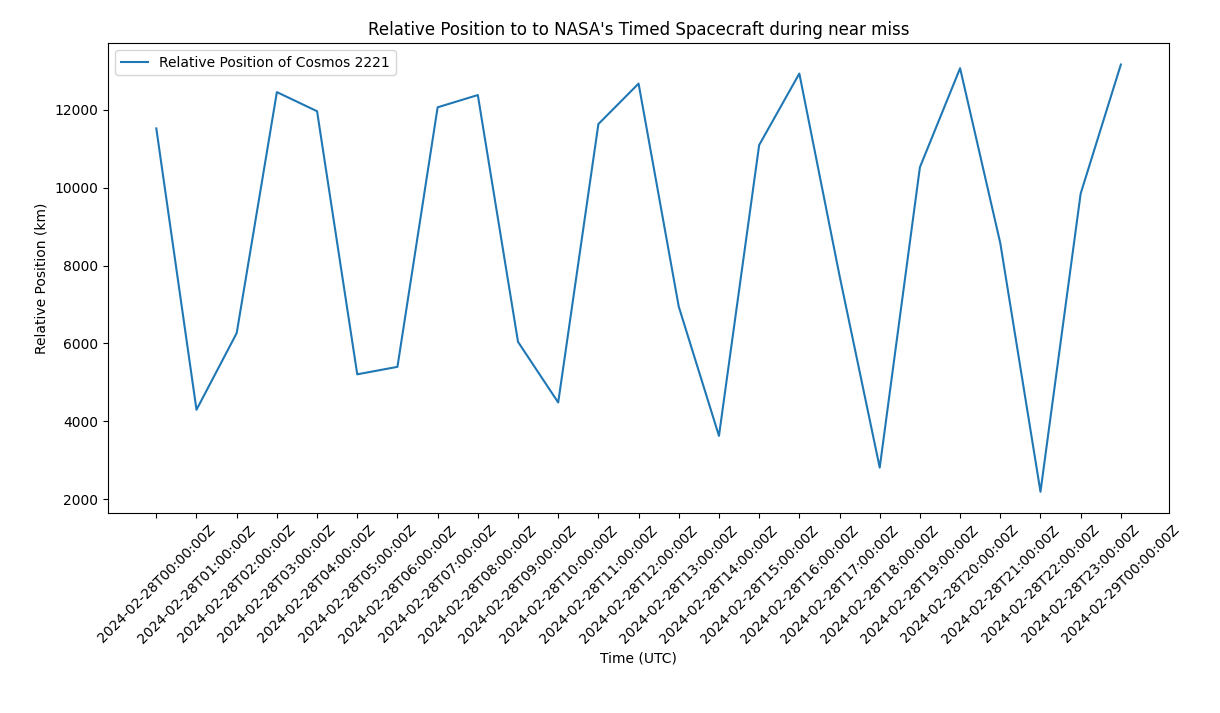
\includegraphics[width=0.8\textwidth]{figure_timed_near_miss.png}
    \caption{Relative position of NASA's Timed satellite and Cosmos 2221 on 2/28/2024}
    \label{fig:orbit}
  \end{figure}


  \textit{Issue:} I tried a real example of a near miss with NASA’s Timed satellite and Cosmos 2221 (with a \textless{}30m distance), but the graphs don’t look accurate. It is weird that the relative position can change 10,000km within hours. The calculations don’t look right.

  \textit{Improve:} I need to cross-check the orbits with GMAT to see the near miss at 6:30 UTC on 2/28/2024. I also need to check if my SGP4 calculations are accurate. Also, could this be a problem with the SGP4 model’s error? Another thing to consider is that TLE’s are updating frequently, the TLE I used is from 5/28/2025.
\end{enumerate}

\chapter*{Next Steps}
\begin{itemize}
  \item Figure out what satellites I want to compare with
  \item Figure out if I am using SGP4 correctly, and that the encountered conditions are correct
  \item Do I need to access old TLEs to see old near misses/collisions?
  \item Cross-check with GMAT
  \item Make my code a usable function so Catherine can just call it. Input? \textrightarrow{} Output (angle and approach speed)
  \item Research about the accuracies of SGP4 and what it actually does
\end{itemize}

\end{document}